\documentclass[a4paper]{article}
\usepackage{amsmath}
\usepackage{amssymb}
\usepackage{braket}%量子力学符号
\usepackage{geometry}
\usepackage{natbib}
\usepackage{float}%稳定图片位置
\usepackage{graphicx,subfig}%画图
\usepackage{caption}
\usepackage[english]{babel}
\usepackage{indentfirst}%缩进
\usepackage{enumerate}%加序号
\usepackage{multirow}%合并行
\usepackage{hyperref}
\usepackage{verbatim}
\title{\Large \textbf{VP390 Problem Set 8}\\
\author{\textbf{Pan, Chongdan ID:516370910121}\\
}
}
\begin{document}
\maketitle
\section{Problem 1}
\noindent
$$U^\dagger U=UU^\dagger=I_n$$
$$\ket{1}=\left(\begin{array}{c}
    0\\1
\end{array}\right)\text{    }\ket{0}=\left(\begin{array}{c}
    1\\0
\end{array}\right)$$

$$\textbf{Pr}(\ket{\psi_1}=\ket{1})=a^2$$
$$\textbf{Pr}(\ket{\psi_1}=\ket{0})=b^2$$


$$\frac{\mathrm{d}U(r)}{\mathrm{d}r}=U_0[-12\frac{a^{12}}{r^{13}}+6(\frac{a^6}{r^7})]=0$$
$$r^6=2a^6\rightarrow r_0=\sqrt[6]{2}a$$
$$U(r_0)=-\frac{U_0}{4}$$
\section{Problem 2}
\begin{enumerate}[(a)]
    \item $$E_{el}=-\frac{1}{4\pi\varepsilon_0}\frac{q_1q_2}{r}+E_{Na+}-E_{Cl-}=-\frac{1.44}{0.24}+5.14-3.62=-4.48\text{eV}$$
    \item $$E_{ex}=|E_{el}|-|E_d|=4.48-4.27=0.21\text{eV}$$
    \item $$E_{ex}=\frac{A}{r^n}=\frac{1}{4\pi\varepsilon_0}\frac{q_1q_2}{r}+E_{Na+}-E_{Cl-}$$
    Since it's in equilibrium position, the two forces are equal
    $$\frac{1}{4\pi\varepsilon_0}\frac{q_1q_2}{r_0^2}=\frac{n}{r_0}\frac{A}{r_0^n}$$
    $$\frac{1.44}{0.24^2}=0.21\frac{n}{0.24}\rightarrow n\approx29,A\approx2.23\times10^{-19}\text{eVnm}^2$$
\end{enumerate}
\section{Problem 3}
$$\rho_{ionic}=er_0=1.6\times10^{-19}\times0.0917\times10^{-9}=1.4672\times10^{-29}\text{Cm}$$
$$\frac{\rho_{measure}}{\rho_{ionic}}=\frac{6.4\times10^{-30}}{1.4672\times10^{-29}}\approx43.6\%$$
\section{Problem 4}
$$\rho_{ionic}=er_0=1.6\times10^{-19}\times0.193\times10^{-9}=3.088\times10^{-29}\text{Cm}$$
$$\frac{\rho_{measure}}{\rho_{ionic}}=\frac{26.7\times10^{-30}}{3.088\times10^{-29}}\approx86.5\%$$
\section{Problem 5}
\begin{enumerate}[(a)]
    \item $$E=h\nu=h\frac{c}{\lambda}\rightarrow\lambda=h\frac{c}{E}=6.63\times10^{-34}\frac{3\times10^8}{0.3\times1.6\times10^{-19}}\approx4.14\times10^{-6}\text{m}$$
    \item Since $\lambda>1000nm$, it belongs to Paschen part of the spectrum, and it's infrared ray
    \item Because the bond strength only accounts for 15\% of the total bond, and others are are not broken
\end{enumerate}
\section{6}
\begin{enumerate}[(a)]
    \item $$\mu=\frac{m_1m_2}{m_1+m_2}=\frac{35.5\times39}{35.3+39}\times1.66\times10^{-27}\approx3.08\times10^{-26}\text{kg}$$
    \item $$I=\frac{\hbar^2}{2E_{rot}}=\frac{(1.05\times10^{-34})^2}{2\times1.43\times10^{-5}\times1.6\times10^{-19}}\approx2.41\times10^{-45}$$
    $$r_0=\sqrt{\frac{I}{\mu}}\approx2.8\times10^{-10}\text{m}$$
\end{enumerate}
\section{7}
$$k=(2\pi f)^2\frac{m_Nm_O}{m_N+m_O}=(2\times\pi\times5.63\times10^{13})^2\frac{14\times16}{14+16}\times1.66\times10^{-27}\approx1551\text{N/m}$$
\section{8}
\begin{enumerate}[(a)]
    \item $$\mu=\frac{m_Cm_O}{m_C+m_O}=\frac{12\times16}{12+16}\times1.66\times10^{-27}\approx1.34\times10^{-26}$$
    $$I=\mu r_0^2=1.34\times10^{-26}\times(0.113\times10^{-9})^2\approx1.45\times10^{-46}kg\cdot m^2$$
    $$E_{0r}=\frac{\hbar^2}{2I}=\frac{(1.05\times10^{-34})^2}{2\times1.45\times10^{-46}}\approx2.37\times10^{-4}\text{eV}$$
    \item $$\omega=\sqrt{\frac{2E_{0r}}{I}}=\sqrt{\frac{2\times2.37\times10^{-4}\times1.6\times10^{-19}}{1.45\times10^{-46}}}\approx7.23\times10^{11}\text{rad/s}$$
    For $\nu=0$:
    $$E_{\nu=0}=\hbar\omega(0+1/2)=1.05\times10^{-34}\times7.23\times10^{11}\times0.5\approx3.8\times10^{-23}\text{J}=2.37\times10^{-4}\text{eV}$$
    Hence for $l=1,\nu=0,E=2.37\times10^{-4}+2\times2.37\times10^{-4}=7.11\times10^{-4}\text{eV}$
    \\For $l=2,\nu=0,E=1.659\times10^{-3}\text{eV}$
    \\For $l=3,\nu=0,E=3.081\times10^{-3}\text{eV}$
    \\For $l=4,\nu=0,E=4.977\times10^{-3}\text{eV}$
    \\For $l=5,\nu=0,E=7.347\times10^{-3}\text{eV}$
    \item
    $\bigtriangleup E_{5\rightarrow 4}=2.37\times10^{-3}\text{eV}$
    \\$\bigtriangleup E_{4\rightarrow 3}=1.896\times10^{-3}\text{eV}$
    \\$\bigtriangleup E_{3\rightarrow 2}=1.422\times10^{-3}\text{eV}$
    \\$\bigtriangleup E_{2\rightarrow 1}=9.48\times10^{-4}\text{eV}$
    \\$\bigtriangleup E_{1\rightarrow 0}=4.74\times10^{-4}\text{eV}$
    \begin{figure}[H]
    \centering
    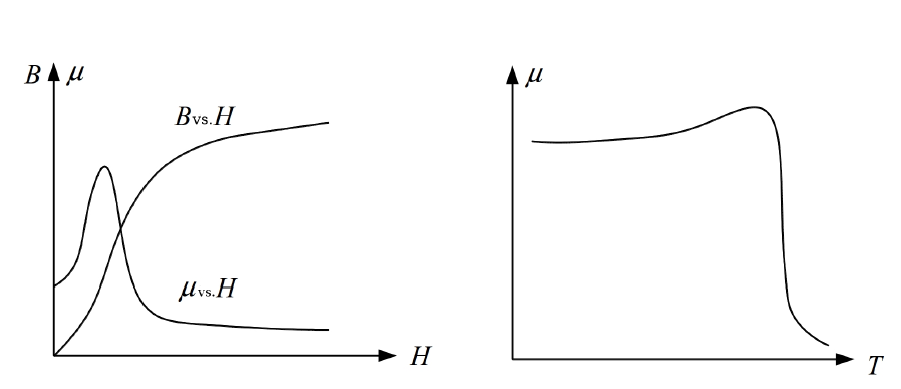
\includegraphics[scale=0.25]{P1.PNG}
    \caption{Energy Diagram when $\nu=0$}
    \end{figure}
    \item $$\lambda_{l+1}=h\frac{c}{E_{l+1\rightarrow l}}=\frac{1.989\times10^{-25}}{1.6\times10^{-19}\times(l+1)(1.05\times10^{-34})^2/(1.45\times10^{-46})}$$
    $$\bigtriangleup \lambda_1=2.62\times10^{-3}\text{m}$$
    $$\bigtriangleup \lambda_2=1.31\times10^{-3}\text{m}$$
    $$\bigtriangleup \lambda_3=8.74\times10^{-3}\text{m}$$
    $$\bigtriangleup \lambda_4=6.56\times10^{-4}\text{m}$$
    $$\bigtriangleup \lambda_5=5.25\times10^{-4}\text{m}$$
    All light are in microwave.
\end{enumerate}
\end{document}